\documentclass{scrartcl}

\usepackage[hidelinks]{hyperref}
\usepackage[none]{hyphenat}
\usepackage{setspace}
\doublespace
\usepackage{multicol}
\usepackage{graphicx}

\title{How does the use of different estimation methods influence the perceived ease of the development process?}
\subtitle{COMP150 - Agile Development Practice}
\author{1702208}
\date{2017-11-08}

\begin{document}

\maketitle{}

\newpage{}

\begin{multicols}{2}

\section{Background}
It is important to make the development process pleasant to work on.
This way a team will be more engaged in the project, which makes it faster to accomplish.
We all know that working without any will never ends well.
Especially estimating and planning in the middle of the project rarely goes perfectly.
In this case, different estimating techniques are useful. 
That is why in this paper I will try to talk about the most engaging ways of estimating.
However, mentioning different levels of planning is a must.

\section{Planning Importance}
In this part, I will try to explain why planning is important for every development project.
But before that, let's consider two variations, which teams respond to.
They either refuse planning or spend too much time on it \cite{cohn2005agile}.
In the first case, it's clear that the team won't be able to answer such questions:
"When will a feature be done?" and "When do we aim to release the product?"
These are some basic questions teams have to have an answer to.
Having no solutions to those will eventually lead to an unproductive process.
And the second one is issued with overplanning.
In this case, overplanning may also cause some major problems.
The team bears in mind that their planning cannot be wrong \cite{cohn2005agile}.
This eventually leads to some unfortunate understandings after realizing that the plan was incorrect.
Therefore, how thoroughly the plan might be it will rarely become more accurate than it should be \cite{cohn2005agile}.
There are a few bits of planning, which you can see in this planning onion.
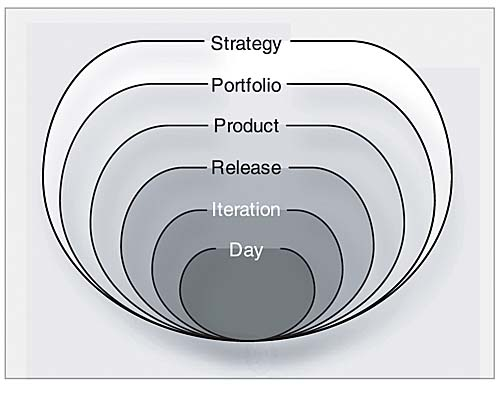
\includegraphics[scale=0.4]{onion}
The most important ones for the development team are daily, iteration and release.
Daily are just casual stand-up meetings we all know well.
But the iteration planning and release planning differ.
First of all, iteration planning is more detailed planning of some features team must do in 1 to 4 weeks.
Whereas release planning is considered for 3 to 6 months.
This includes what features should be implemented by the given time \cite{grenning2002planning}.
Although this type of planning shouldn't be left somewhere on the top of a shelf.
It is recommended that release planning is overviewed and changed every time an iteration ends.
So, after all this, it's time to make clear why planning is important.
Planning is a way to optimally answer this one question: What should we build? \cite{cohn2005agile}
Moreover, a good planning should include such options:
Reducing risk \cite{grapenthin2016supporting}, reducing uncertainty, supporting better decision making, establishing trust, conveying information.
To better understand these, see Mike Cohn's book "Agile Estimating and Planning" Chapter 1.

\section{Estimating Backlog}
So, once we have discussed planning, let's jump into estimating.
In an agile development company estimating backlog has a unique place.
Talking specifically about agile game development, estimating user stories is nonetheless important.
An agile development team has to know how much a story is worth.
By saying that, I mean whether a particular feature is difficult to implement or not.
For different people, it might take different time.
One could implement it in a 2-day length, whereas another can do that in 5 days.
That is the main purpose of estimating stories.
Although there are two types of estimating points: story points and ideal days \cite{cohn2005agile}.
Story points are preferred, but for novice teams, ideal days are easier.
Ideal days mean working hours excluding breaks and other difficulties.
On the other side, story points are just points, which should be considered as:
Is this user story harder (or easier) to implement than the previous one?
For example, a story was estimated with 4 story points.
And the next user story is considered a little bit easier to implement, that means it's worth 3 story points.
Advanced teams prefer this type of estimation because they can easily divide those equally for each day.
It is a good way of planning iterations \cite{haugen2006empirical}.
But sometimes teams run into some problems, which eventually cause time waste.
The first one is that not every member of a team is participating.
This only means they are not enjoying the estimation.
The other problem is that it takes too much worthwhile time \cite{cunningham2005costs}.
But, there is a solution - planning poker!

\section{Planning Poker}
First things first, planning poker is an engaging way of estimating user stories.
Some stories don't take much time \cite{grenning2002planning} and discussions make clear why it was estimated exactly this way \cite{cohn2005agile}.
Moreover, there are a couple ways of playing this small game.
User stories can either be estimated by non-linear numbers or poker chips.
Each of these has its own unique level of engagement \cite{molokken2007combining}.
First of all, non-linear numbers - also called Fibonacci scale \cite{tamrakar2012does}.
Those are 0, 1, 2, 3, 5, 8, 13, 20, 40 and 100.
The idea for Fibonacci scale is that people are biased taking the average.
And the median of this scale is considered 8, whereas a linear scales is 20 \cite{tamrakar2012does}.
When playing planning poker with this type of estimation, numbers usually represent working hours.
It's somewhat helpful, but not as engaging as playing with poker chips.
The way poker chips sound when placing onto a table makes people become emotionally engaged \cite{yip2007hands}.
In general, stakeholders can buy a story which they want to be implemented in the next iteration.
To understand it in more detail, see \cite{yip2007hands}.
So, these types are definitely somewhat physically and emotionally engaging.
Thus, team's mental engagement increases \cite{yip2007hands}.
And how do we use this in agile game development? 
Simply as it is, after estimating user stories, the product owner can decide what stories are worth implementing first.
Rather than discussing each story and getting to no conclusion, this is much easier.

\section{Conclusion}
So, does different estimating techniques provide a more easy way of development?
It surely does; after all, it is hard to work continuously without having any fun.
And that is why agile teams usually play planning poker to increase members' engagement.
Furthermore, as this paper discusses, it helps to plan iterations, which are nonetheless important.
Let's briefly remember all the important things.
First of all, iterations help teams plan what features should be done in a 1 to 4 week time.
Iterations show features in more details, which, of course, helps the team to implement it faster.
Whereas release planning is more for a business purpose that lasts for 3 to 6 months.
This should answer such question as: "When will the product be released?"
It can also be changed depending on what features the product owner wants to see.
For example, it sometimes worth implementing more features, but a bit later... or the other way.
About estimating I can only claim that it helps the team to understand a feature's importance.
As it sometimes becomes boring, planning poker is a great solution to make it interesing.
It surely increases team's mental engagement into the project.

\end{multicols}

\bibliography{References}
\bibliographystyle{ieeetr}

\end{document}

To make it more engaging there are some entertaining methods of estimating backlog, which I will introduce later in this paper.
there are a couple ways of engaging planning poker.